
% This section uses TikZ figures. Ensure the preamble includes: \usepackage{tikz}

\section{Diffusion Models: Mathematical Formulation}

The previous section introduced diffusion conceptually as generation by repeated denoising.
We now make that picture precise.
This section is one of the mathematical anchors of the chapter: it states the forward Markov chain exactly, derives the Gaussian marginals and posterior conditionals that make training tractable, and explains why the practical noise-prediction objective is a simplified variational objective rather than an unrelated heuristic.

\medskip

\noindent
\textbf{Guiding question.}
How can one turn a fixed corruption process into a trainable generative model whose reverse dynamics map simple noise back to structured data?

\subsection*{The formal forward Markov chain}

Let $x_0\in\mathbb{R}^d$ denote a clean data point.
A discrete-time diffusion model begins by fixing a noising schedule $\beta_1,\dots,\beta_T$ with $0<\beta_t<1$, and defining
\[
\alpha_t = 1-\beta_t,
\qquad
\bar\alpha_t = \prod_{s=1}^t \alpha_s.
\]

\begin{definition}[Forward diffusion chain]
The forward process is the Markov chain
\[
q(x_{1:T}\mid x_0)=\prod_{t=1}^T q(x_t\mid x_{t-1}),
\]
with Gaussian transitions
\[
q(x_t\mid x_{t-1})
=
\mathcal{N}\!\bigl(x_t\mid \sqrt{\alpha_t}\,x_{t-1},\,\beta_t I\bigr).
\]
\end{definition}

Each step preserves most of the current signal but injects a small amount of Gaussian noise.
When $T$ is large enough and the schedule is chosen appropriately, the terminal variable $x_T$ is close to an isotropic Gaussian.
The fixed forward chain is exact; no learning enters here.

\begin{figure}[h]
\centering
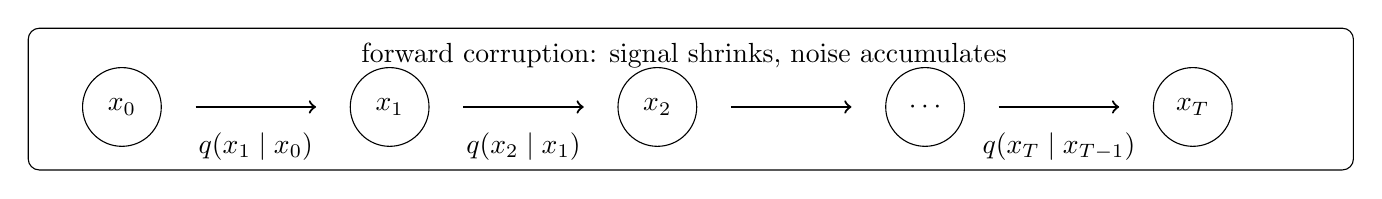
\begin{tikzpicture}[x=1.7cm,y=1cm]
    \draw[rounded corners] (-0.7,-0.8) rectangle (9.2,1.0);
    \node at (0,0) [draw,circle,minimum size=1cm] {$x_0$};
    \node at (2,0) [draw,circle,minimum size=1cm] {$x_1$};
    \node at (4,0) [draw,circle,minimum size=1cm] {$x_2$};
    \node at (6,0) [draw,circle,minimum size=1cm] {$\cdots$};
    \node at (8,0) [draw,circle,minimum size=1cm] {$x_T$};
    \draw[->,thick] (0.55,0) -- (1.45,0);
    \draw[->,thick] (2.55,0) -- (3.45,0);
    \draw[->,thick] (4.55,0) -- (5.45,0);
    \draw[->,thick] (6.55,0) -- (7.45,0);
    \node at (1,-0.5) {$q(x_1\mid x_0)$};
    \node at (3,-0.5) {$q(x_2\mid x_1)$};
    \node at (7,-0.5) {$q(x_T\mid x_{T-1})$};
    \node at (4.2,0.65) {forward corruption: signal shrinks, noise accumulates};
\end{tikzpicture}
\caption{The forward diffusion chain is a fixed Gaussian Markov process that gradually destroys structure.}
\end{figure}

\subsection*{Closed-form forward marginals}

The usefulness of the Gaussian forward chain lies in the fact that one can move from $x_0$ to any intermediate time $t$ in closed form.
This is what makes training efficient.

\begin{proposition}[Closed-form forward marginal]
For the forward chain above,
\[
q(x_t\mid x_0)
=
\mathcal{N}\!\left(x_t\mid \sqrt{\bar\alpha_t}\,x_0,\, (1-\bar\alpha_t)I\right).
\]
Equivalently,
\[
x_t = \sqrt{\bar\alpha_t}\,x_0 + \sqrt{1-\bar\alpha_t}\,\varepsilon,
\qquad \varepsilon\sim \mathcal{N}(0,I).
\]
\end{proposition}

\begin{proof}
We argue by induction on $t$.
For $t=1$ the claim is exactly the definition of $q(x_1\mid x_0)$.
Assume
\[
x_{t-1}=\sqrt{\bar\alpha_{t-1}}\,x_0 + \sqrt{1-\bar\alpha_{t-1}}\,\varepsilon_{t-1},
\qquad \varepsilon_{t-1}\sim \mathcal{N}(0,I).
\]
From the transition equation,
\[
x_t = \sqrt{\alpha_t}\,x_{t-1} + \sqrt{\beta_t}\,z_t,
\qquad z_t\sim\mathcal{N}(0,I).
\]
Substituting the induction hypothesis gives
\[
x_t = \sqrt{\alpha_t\bar\alpha_{t-1}}\,x_0
+ \sqrt{\alpha_t(1-\bar\alpha_{t-1})}\,\varepsilon_{t-1}
+ \sqrt{\beta_t}\,z_t.
\]
Because the last two terms are independent centered Gaussians, their sum is Gaussian with covariance
\[
\alpha_t(1-\bar\alpha_{t-1})I + \beta_t I
=
(1-\alpha_t\bar\alpha_{t-1})I
=
(1-\bar\alpha_t)I.
\]
Also $\alpha_t\bar\alpha_{t-1}=\bar\alpha_t$, so the mean is $\sqrt{\bar\alpha_t}\,x_0$.
This proves the claim.
\end{proof}

\noindent
\textbf{Interpretation.}
The entire history $x_1,\dots,x_{t-1}$ can be collapsed into a single effective corruption level.
Training therefore does not require simulating the whole chain step by step.
One may sample a time index $t$, draw one Gaussian noise vector $\varepsilon$, and construct $x_t$ directly.

\subsection*{Posterior conditionals and reverse-process parameterization}

To learn generation, one would ideally model the exact reverse conditionals induced by the forward chain.
For the Gaussian process above, the relevant posterior is itself Gaussian when conditioned on both $x_t$ and the original $x_0$.

\begin{proposition}[Gaussian posterior for one reverse step]
For $t\ge 1$,
\[
q(x_{t-1}\mid x_t,x_0)
=
\mathcal{N}\!\bigl(x_{t-1}\mid \tilde\mu_t(x_t,x_0),\,\tilde\beta_t I\bigr),
\]
where
\[
\tilde\beta_t = \frac{1-\bar\alpha_{t-1}}{1-\bar\alpha_t}\,\beta_t,
\]
and
\[
\tilde\mu_t(x_t,x_0)
=
\frac{\sqrt{\bar\alpha_{t-1}}\,\beta_t}{1-\bar\alpha_t}\,x_0
+
\frac{\sqrt{\alpha_t}(1-\bar\alpha_{t-1})}{1-\bar\alpha_t}\,x_t.
\]
\end{proposition}

\begin{proof}[Proof sketch]
Use Bayes' rule with the two Gaussian factors
\[
q(x_t\mid x_{t-1})
\qquad \text{and} \qquad
q(x_{t-1}\mid x_0).
\]
Their product, viewed as a function of $x_{t-1}$, is proportional to a Gaussian density.
Completing the square yields the stated posterior mean and variance.
\end{proof}

This proposition explains why the reverse model is commonly parameterized as
\[
p_\theta(x_{0:T}) = p(x_T)\prod_{t=1}^T p_\theta(x_{t-1}\mid x_t),
\qquad p(x_T)=\mathcal{N}(0,I),
\]
with Gaussian reverse transitions
\[
p_\theta(x_{t-1}\mid x_t)
=
\mathcal{N}\!\bigl(x_{t-1}\mid \mu_\theta(x_t,t),\,\Sigma_\theta(x_t,t)\bigr).
\]
The true reverse conditional depends on the unknown $x_0$, so the network must infer from $x_t$ what clean structure likely produced the noisy observation.

A standard and extremely useful parameterization predicts the noise rather than the mean directly.
If a network $\varepsilon_\theta(x_t,t)$ estimates the forward noise, then one defines
\[
\hat x_0(x_t,t)
=
\frac{x_t-\sqrt{1-\bar\alpha_t}\,\varepsilon_\theta(x_t,t)}{\sqrt{\bar\alpha_t}},
\]
and substitutes $\hat x_0$ into the posterior-mean formula.
Equivalently, when the reverse variance is chosen as a fixed known schedule,
\[
\mu_\theta(x_t,t)
=
\frac{1}{\sqrt{\alpha_t}}
\left(
 x_t - \frac{\beta_t}{\sqrt{1-\bar\alpha_t}}\,\varepsilon_\theta(x_t,t)
\right).
\]
Thus reverse-process learning can be organized around estimating either $x_0$, the reverse mean, or the forward noise; these are different parameterizations of the same Gaussian structure.

\subsection*{A clean variational decomposition}

Diffusion training admits a variational derivation analogous in spirit to the ELBO for latent-variable models.
Here the latent variables are the intermediate noise states $x_1,\dots,x_T$.
For a datapoint $x_0$, define
\[
\mathcal{L}_{\mathrm{vlb}}(x_0;\theta)
=
\mathbb{E}_{q(x_{1:T}\mid x_0)}
\left[
\log q(x_{1:T}\mid x_0) - \log p_\theta(x_{0:T})
\right].
\]
Then
\[
-\log p_\theta(x_0)
\le
\mathcal{L}_{\mathrm{vlb}}(x_0;\theta),
\]
so minimizing $\mathcal{L}_{\mathrm{vlb}}$ maximizes a lower bound on the log-likelihood.

Expanding the chain terms gives the decomposition
\begin{align*}
\mathcal{L}_{\mathrm{vlb}}(x_0;\theta)
&=
D_{\mathrm{KL}}\!\bigl(q(x_T\mid x_0)\,\|\,p(x_T)\bigr)
\\
&\quad + \sum_{t=2}^{T}
\mathbb{E}_{q(x_t\mid x_0)}
\left[
D_{\mathrm{KL}}\!\bigl(q(x_{t-1}\mid x_t,x_0)\,\|\,p_\theta(x_{t-1}\mid x_t)\bigr)
\right]
\\
&\quad - \mathbb{E}_{q(x_1\mid x_0)}\bigl[\log p_\theta(x_0\mid x_1)\bigr].
\end{align*}

\noindent
\textbf{Interpretation.}
This formula separates the training problem into three parts:
matching the terminal noise distribution to a simple Gaussian prior, matching each learned reverse step to the exact Gaussian posterior, and reconstructing the final clean sample from a slightly noisy version.
The first term is usually fixed by design, the middle terms are the main diffusion-specific KL penalties, and the last term acts like a data-reconstruction term.

\subsection*{From the variational bound to the noise-prediction objective}

The practical success of diffusion models depends on the fact that the complicated variational objective above reduces to a very simple supervised denoising objective under common parameter choices.

Suppose the reverse variance is fixed and only the mean is learned.
Then each intermediate KL term becomes, up to constants independent of $\theta$,
\[
\mathbb{E}\Bigl[\|\tilde\mu_t(x_t,x_0)-\mu_\theta(x_t,t)\|^2\Bigr].
\]
If we use the noise parameterization of $\mu_\theta$, then the mean-matching loss becomes a weighted noise-prediction loss.

\begin{proposition}[Simplified objective under noise parameterization]
If $p_\theta(x_{t-1}\mid x_t)$ is Gaussian with fixed variance $\tilde\beta_t I$ and mean parameterized by $\varepsilon_\theta(x_t,t)$ as above, then each variational term satisfies
\[
L_t
=
\mathbb{E}_{x_0,\varepsilon}
\left[
\frac{\beta_t^2}{2\tilde\beta_t\alpha_t(1-\bar\alpha_t)}
\,\|\varepsilon-\varepsilon_\theta(x_t,t)\|^2
\right] + C_t,
\]
where $x_t=\sqrt{\bar\alpha_t}x_0+\sqrt{1-\bar\alpha_t}\,\varepsilon$ and $C_t$ does not depend on $\theta$.
\end{proposition}

\begin{proof}[Proof sketch]
The KL between two Gaussians with the same covariance is proportional to the squared distance between their means.
Substitute the exact posterior mean $\tilde\mu_t(x_t,x_0)$ and the parameterized mean $\mu_\theta(x_t,t)$.
After algebraic simplification, the difference between the two means is a known scalar multiple of $\varepsilon-\varepsilon_\theta(x_t,t)$.
The stated coefficient is exactly the square of that scalar divided by the Gaussian variance term appearing in the KL.
\end{proof}

This is the origin of the standard training objective
\[
\mathcal{L}_{\mathrm{simple}}(\theta)
=
\mathbb{E}_{x_0,\varepsilon,t}
\left[
\|\varepsilon-\varepsilon_\theta(x_t,t)\|^2
\right],
\qquad
x_t=\sqrt{\bar\alpha_t}x_0+\sqrt{1-\bar\alpha_t}\,\varepsilon.
\]
Strictly speaking, this objective omits time-dependent weights and certain auxiliary terms from the full variational bound.
Empirically, however, it works extremely well and is the training rule most readers encounter first.

\subsection*{Relation to score matching}

Diffusion is closely related to score-based generative modeling.
Recall that the score of a density $p$ is
\[
\nabla_x \log p(x).
\]
For the Gaussian corruption model,
\[
q(x_t\mid x_0)=\mathcal{N}\!\left(x_t\mid \sqrt{\bar\alpha_t}x_0,(1-\bar\alpha_t)I\right),
\]
so the conditional score is explicit.

\begin{proposition}[Noise prediction and conditional score estimation]
For fixed $x_0$ and $t$,
\[
\nabla_{x_t}\log q(x_t\mid x_0)
=
-\frac{x_t-\sqrt{\bar\alpha_t}x_0}{1-\bar\alpha_t}
=
-\frac{\varepsilon}{\sqrt{1-\bar\alpha_t}}.
\]
Hence predicting $\varepsilon$ is equivalent, up to a known scalar factor, to predicting the conditional score of the noisy distribution.
\end{proposition}

\begin{proof}
Differentiate the log-density of the Gaussian $q(x_t\mid x_0)$ with respect to $x_t$.
Then substitute
\[
x_t-\sqrt{\bar\alpha_t}x_0=\sqrt{1-\bar\alpha_t}\,\varepsilon.
\]
\end{proof}

This proposition does not say that the network directly learns the unconditional score $\nabla_{x_t}\log q_t(x_t)$ in exactly this form.
Rather, it explains why denoising and score estimation are so closely connected: once Gaussian perturbations are introduced, the direction in which one should move to increase data density is encoded in the same residual term that appears in the denoising task.

\subsection*{DDPM and DDIM as formal sampling viewpoints}

The same trained denoiser can support different reverse-time samplers.
Two important viewpoints are DDPM and DDIM.

\paragraph{DDPM.}
In the original diffusion probabilistic model, sampling is stochastic.
At time $t$, one forms $\hat x_0$ from the predicted noise, computes the reverse mean $\mu_\theta(x_t,t)$, and samples
\[
x_{t-1} \sim \mathcal{N}\!\bigl(\mu_\theta(x_t,t),\,\sigma_t^2 I\bigr),
\]
with $\sigma_t^2$ chosen from the variance schedule.
This closely follows the probabilistic reverse-chain interpretation.

\paragraph{DDIM.}
DDIM keeps the same training objective but uses a non-Markovian sampling construction that can be written as
\[
x_{t-1}
=
\sqrt{\bar\alpha_{t-1}}\,\hat x_0
+
\sqrt{1-\bar\alpha_{t-1}-\sigma_t^2}\,\hat\varepsilon
+
\sigma_t z,
\]
where $\hat\varepsilon=\varepsilon_\theta(x_t,t)$, $z\sim\mathcal{N}(0,I)$, and $\sigma_t$ is chosen by the sampler.
Setting $\sigma_t=0$ gives a deterministic update.

\medskip

\noindent
\textbf{Formal comparison.}
DDPM is a stochastic approximation to the reverse diffusion chain and naturally emphasizes probabilistic sampling.
DDIM uses the same learned denoiser but chooses a family of trajectories consistent with the same training objective, including deterministic ones.
Thus the model is the learned denoiser; the sampler is a separate algorithmic choice built on top of it.

\begin{figure}[h]
\centering
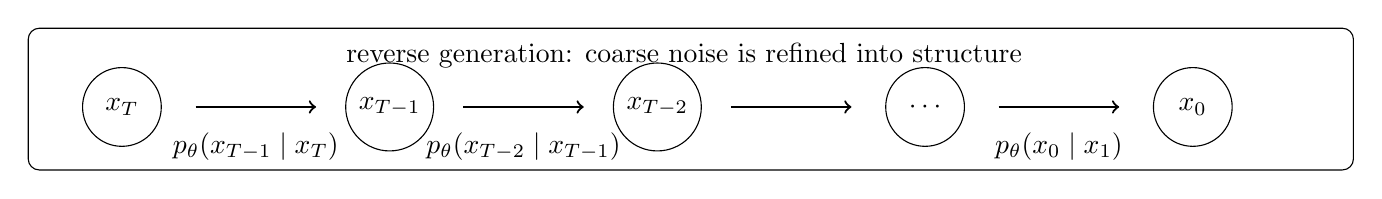
\begin{tikzpicture}[x=1.7cm,y=1cm]
    \draw[rounded corners] (-0.7,-0.8) rectangle (9.2,1.0);
    \node at (0,0) [draw,circle,minimum size=1cm] {$x_T$};
    \node at (2,0) [draw,circle,minimum size=1cm] {$x_{T-1}$};
    \node at (4,0) [draw,circle,minimum size=1cm] {$x_{T-2}$};
    \node at (6,0) [draw,circle,minimum size=1cm] {$\cdots$};
    \node at (8,0) [draw,circle,minimum size=1cm] {$x_0$};
    \draw[->,thick] (0.55,0) -- (1.45,0);
    \draw[->,thick] (2.55,0) -- (3.45,0);
    \draw[->,thick] (4.55,0) -- (5.45,0);
    \draw[->,thick] (6.55,0) -- (7.45,0);
    \node at (1,-0.5) {$p_\theta(x_{T-1}\mid x_T)$};
    \node at (3,-0.5) {$p_\theta(x_{T-2}\mid x_{T-1})$};
    \node at (7,-0.5) {$p_\theta(x_0\mid x_1)$};
    \node at (4.2,0.65) {reverse generation: coarse noise is refined into structure};
\end{tikzpicture}
\caption{A learned reverse chain maps a simple Gaussian terminal state back to data. DDPM uses stochastic steps; DDIM can use deterministic ones.}
\end{figure}

\subsection*{Worked one-dimensional example}

Consider the one-dimensional case with $T=1$ and variance schedule $\beta_1=0.36$, so $\alpha_1=0.64$ and $\bar\alpha_1=0.64$.
Then
\[
q(x_1\mid x_0)=\mathcal{N}(x_1\mid 0.8x_0,0.36).
\]
If $x_0=2$ and the sampled forward noise is $\varepsilon=-1$, then
\[
x_1 = 0.8\cdot 2 + 0.6(-1)=1.0.
\]
Suppose a denoiser predicts $\varepsilon_\theta(x_1,1)=-0.9$.
Then the reconstructed clean sample is
\[
\hat x_0
=
\frac{x_1-\sqrt{1-\bar\alpha_1}\,\varepsilon_\theta(x_1,1)}{\sqrt{\bar\alpha_1}}
=
\frac{1.0-0.6(-0.9)}{0.8}
=1.925.
\]
The noise-prediction loss for this single example is
\[
(\varepsilon-\varepsilon_\theta)^2 = (-1+0.9)^2 = 0.01.
\]
Even in this tiny example one sees the basic logic: the model never receives the exact posterior; it learns to infer what noise must have been added, and that estimate is enough to reconstruct an approximation of the clean data point.

\subsection*{What is exact, approximate, and heuristic}

The mathematical structure of diffusion is unusually clean, but different parts of the method live at different levels of certainty.

\begin{itemize}
    \item \textbf{Exact:} the forward Gaussian chain, its closed-form marginals, and the Gaussian posterior formulas are exact consequences of the chosen corruption process.
    \item \textbf{Variationally justified:} the reverse-chain likelihood bound and the resulting KL decomposition are exact identities once the forward process and reverse family are specified.
    \item \textbf{Approximate but principled:} the learned reverse conditionals are approximations to the true reverse conditionals, and the simplified noise-prediction loss drops weights and terms from the full variational objective.
    \item \textbf{Design practice:} noise schedules, sampler choices, parameterizations, architectural details, and acceleration rules remain partly empirical.
\end{itemize}

This separation matters pedagogically.
The elegance of diffusion does not come from pretending every successful implementation detail is theoretically inevitable.
It comes from recognizing that a large and useful class of those details sits on top of a remarkably transparent probabilistic core.

\subsection*{What to remember}

\begin{itemize}
    \item The forward diffusion process is a fixed Gaussian Markov chain with closed-form marginals.
    \item The reverse model learns Gaussian conditionals intended to approximate the true reverse posterior steps.
    \item The diffusion ELBO decomposes into terminal, reverse-step, and reconstruction terms.
    \item The practical noise-prediction loss is a simplified variational objective.
    \item Diffusion is closely connected to score estimation on noisy data.
\end{itemize}

\subsection*{Common confusion}

\begin{itemize}
    \item Predicting noise is not a separate idea from reverse-process learning; it is a convenient parameterization of it.
    \item The forward process is not learned in the standard formulation.
    \item DDPM and DDIM differ mainly in sampling dynamics, not in the fundamental denoiser-training objective.
    \item A simplified training loss can still be principled even if it is not the full likelihood objective written term by term.
\end{itemize}

\subsection*{Exercises}

\begin{enumerate}
    \item Prove the closed-form forward marginal again, but this time by composing Gaussian means and covariances recursively rather than using the explicit noise representation.
    \item Starting from the Gaussian formula for $q(x_t\mid x_{t-1})$ and the closed-form formula for $q(x_{t-1}\mid x_0)$, derive the posterior $q(x_{t-1}\mid x_t,x_0)$ by completing the square.
    \item Show directly that the conditional score formula
    \[
    \nabla_{x_t}\log q(x_t\mid x_0) = -\frac{\varepsilon}{\sqrt{1-\bar\alpha_t}}
    \]
    follows from the Gaussian density and the reparameterized form of $x_t$.
    \item Explain in words why the simplified noise-prediction objective can be interpreted as supervised learning, even though the overall model is generative.
    \item Compare DDPM and DDIM from the viewpoint of stochastic versus deterministic trajectories. What remains common between them?
\end{enumerate}

\subsection*{Notes and references}

The modern discrete-time diffusion formulation was developed in the diffusion probabilistic-model literature and later clarified and generalized through score-based generative-model work.
Important reference points include denoising score matching, diffusion probabilistic models, improved DDPM-style training, and DDIM-style non-stochastic sampling.
Conceptually, the section also inherits ideas from denoising autoencoders, variational latent-variable modeling, and stochastic-process viewpoints on generation.
